%% Author - Varad Meru
%% tex source file for Homework 1.
%%%%%%%%%%%%%%%%%%%%%%%%%%%%%%%%%%%%%%%%%%%%%%%%%%%%%%%%%
%%%%%%%%%%%%%%%%%%%%%%%%%%%%%%%%%%%%%%%%%%%%%%%%%%%%%%%%%
\documentclass[a4paper, 11pt]{article}

\usepackage[margin=1in]{geometry} % changes the margin
\usepackage{lipsum} % adds random text to check the formatting
\usepackage{hyperref} % adds hyperlink
\usepackage[framed,numbered,autolinebreaks,useliterate]{mcode}
\usepackage{subfigure}
\usepackage{graphicx}
\usepackage{enumerate}

\renewcommand{\thefootnote}{\fnsymbol{footnote}} % Changes the format of the footnotes superscripts

%%%%%%%%%%%%%%%%%%%%%%%%%%%%%%%%%%%%%%%%%%%%%%%%%%%%%%%%%
\begin{document}
\begin{noindent}
\large\textbf{Week 1} \hfill \textbf{Varad Meru} \\
\normalsize CS 273a - Introduction to Machine Learning (Winter '15)\footnote{\href{http://sli.ics.uci.edu/Classes/2015W-273a}{Website: http://sli.ics.uci.edu/Classes/2015W-273a}} \hfill Student \# 26648958 \\
Prof. Alex Ihler \hfill Due Date: 01/13/2015
\end{noindent}
\noindent\makebox[\linewidth]{\rule{\textwidth}{0.4pt}}

%%%%%%%%%%%%%%%%%%%%%%%%%%%%%%%%%%%%%%%%%%%%%%%%%%%%%%%%%
%%%%%%%%%%%%%%%%%%%%%%%%%%%%%%%%%%%%%%%%%%%%%%%%%%%%%%%%%
\begin{center}
\textbf{\Large{Homework 1}\footnote{Questions available at \href{http://sli.ics.uci.edu/Classes/2015W-273a?action=download&upname=HW1.pdf}{http://sli.ics.uci.edu/Classes/2015W-273a?action=download\&upname=HW1.pdf}}\footnote{All the figures and listing numbers are auto-refered.}}\\
\end{center}
\vspace{-25pt}

%%%%%%%%%%%%%%%%%%%%%%%%%%%%%%%%%%%%%%%%%%%%%%%%%%%%%%%%%
%%%%%%%%%%%%%%%%%%%%%%%%%%%%%%%%%%%%%%%%%%%%%%%%%%%%%%%%%
\section*{Problem 1: Matlab \& Data Exploration}
\vspace{-5pt}
In this problem, I looked at some constructs provided by Matlab to perform basic statistics and get visualizations of an example data set. I used the downloaded and loaded the \textit{Fisher iris} dataset provided using code given in \autoref{lst:loadListing}.
\vspace{-15pt}
\begin{lstlisting}[caption={Load iris data set and create necessary variables},label={lst:loadListing},numbers=left,escapeinside={@}{@}]
% Fetching the dataset and separating it into X and Y.
iris=load('data/iris.txt');     % load the text file
y = iris(:,end);           % target value is last column
X = iris(:,1:end-1);       % features are other columns
features = char('Sepal length','Sepal width','Petal length','Petal width','Species');
features_short = char('SL','SW','PL','PW','SP');
disp(whos);

% Changed the shuffleData function to take a seed from the user. If not
% provided, then it generates it randomly.
[X, y] = shuffleData(X,y,s);

% Used in some sub-problems
X = X(:,1:2);
[Xtr,Xte,Ytr,Yte] = splitData(X,y, .75);
\end{lstlisting}

I have listed the approaches I used for solving the sub-parts of the problem. This question had six sub-parts.
\begin{enumerate}[(a)]
\item The size of the data matrix X is computed using the \mcode{size()} function provided by Matlab.
\vspace{-30pt}
\begin{lstlisting}[caption={Displaying the size of input matrix X. output written in the next line of the command},label={lst:hist1Listing},numbers=left,escapeinside={@}{@}]
% Part (a) - Use size(X,2) to get the number of features, and size(X,1) to get the number of data points.
disp(size(X, 1));
   148
disp(size(X, 2));
     2
\end{lstlisting}

\item For plotting the histograms for each feature, I used the \mcode{histogram()} function provided by Matlab as shown in \autoref{lst:hist1Listing}. You can see the histograms in \autoref{fig:histogram1a}. The saves function is used to store the produced histograms as image files. \autoref{fig:histogram1b} shows a unified view of all the features of the dataset overlapped.
\vspace{-20pt}
\begin{lstlisting}[caption={Matlab code for creating histograms.},label={lst:hist1Listing},numbers=left,escapeinside={@}{@}]
%% Part (b)
% For each feature, plot a histogram ("hist") of the data values
for f=1:size(X, 2);
    h=figure;
    %subplot(1,4,f)
    h1=histogram(X(:,f)); % histogram is preferred over hist - matlab documentation
    title(strcat('Feature:- ',features(f,:)))
    %hold on;
    saveas(h,strcat('histogram',num2str(f)),'jpg');
end;
%hold off;
\end{lstlisting}
\vspace{-20pt}
\begin{lstlisting}[caption={Overlapping histograms to show a unified view of  `Fisher iris' dataset.},label={lst:hist2Listing},numbers=left,escapeinside={@}{@}]
% All in one
h=figure;
for f=1:size(X, 2);
    histogram(X(:,f));
    hold on;
end;
hold off;
saveas(h,'histogram5.jpg','jpg');
\end{lstlisting}

\begin{figure}
\centering
\subfigure[Sepal Length]{
    \label{fig:subfig1}
    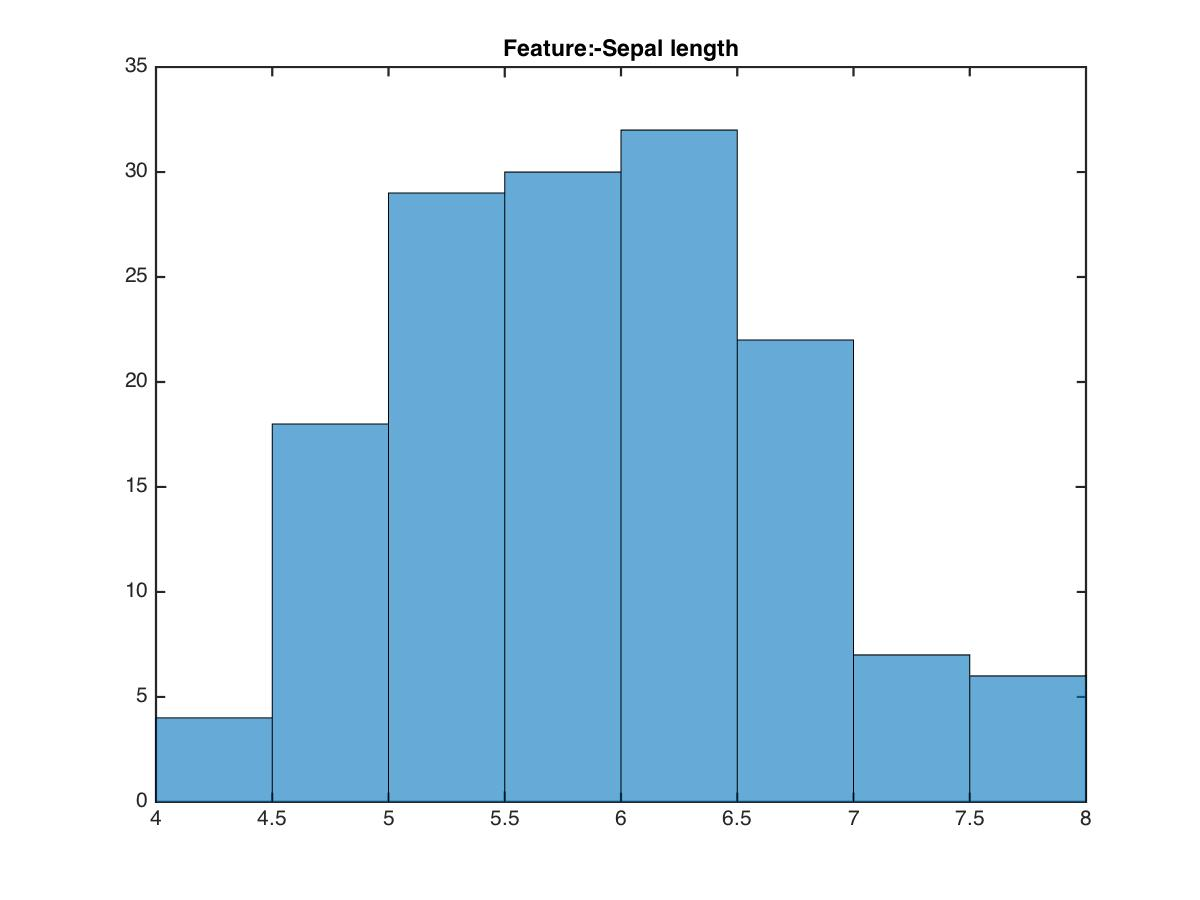
\includegraphics[scale=0.18]{histogram1.jpg}
}
\subfigure[Sepal Width]{
    \label{fig:subfig2}
    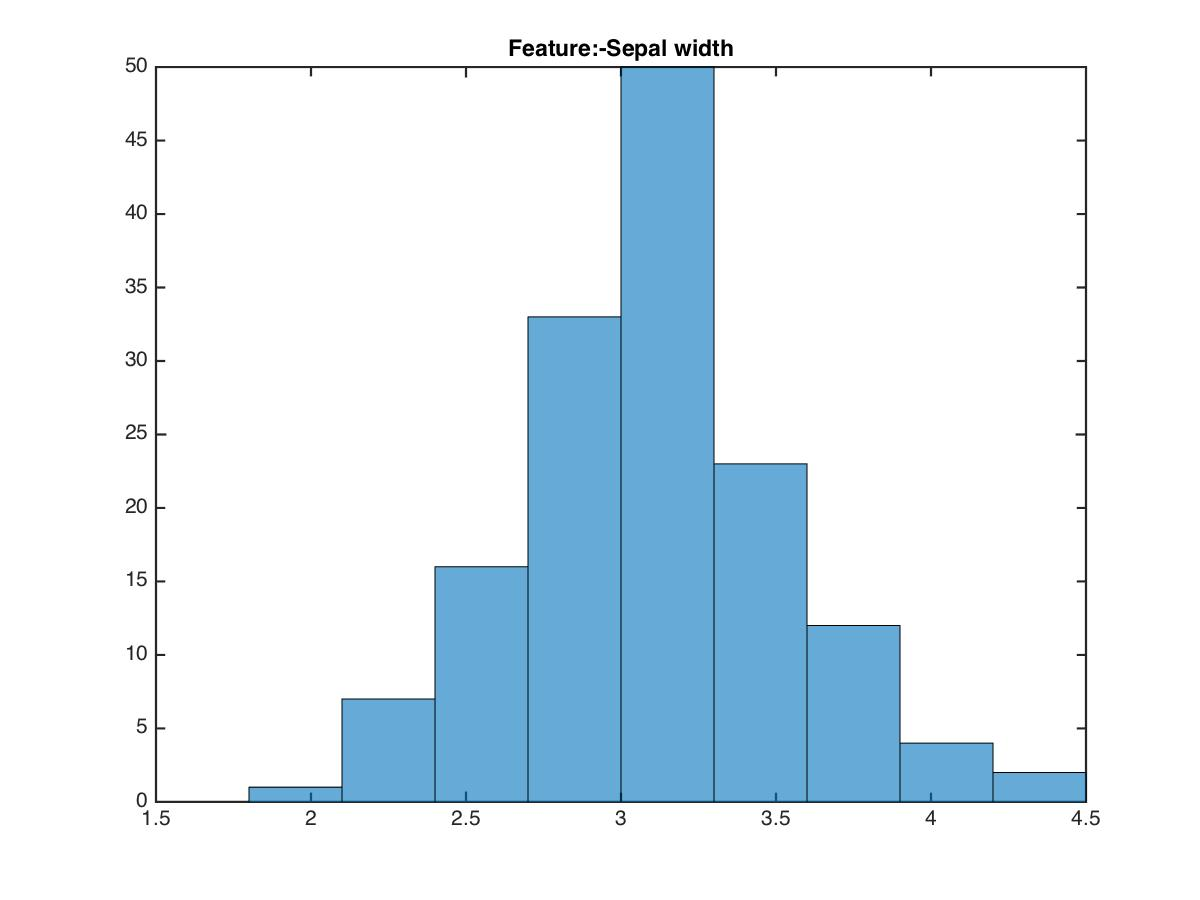
\includegraphics[scale=0.18]{histogram2.jpg}
}
\subfigure[Petal Length]{
    \label{fig:subfig3}
    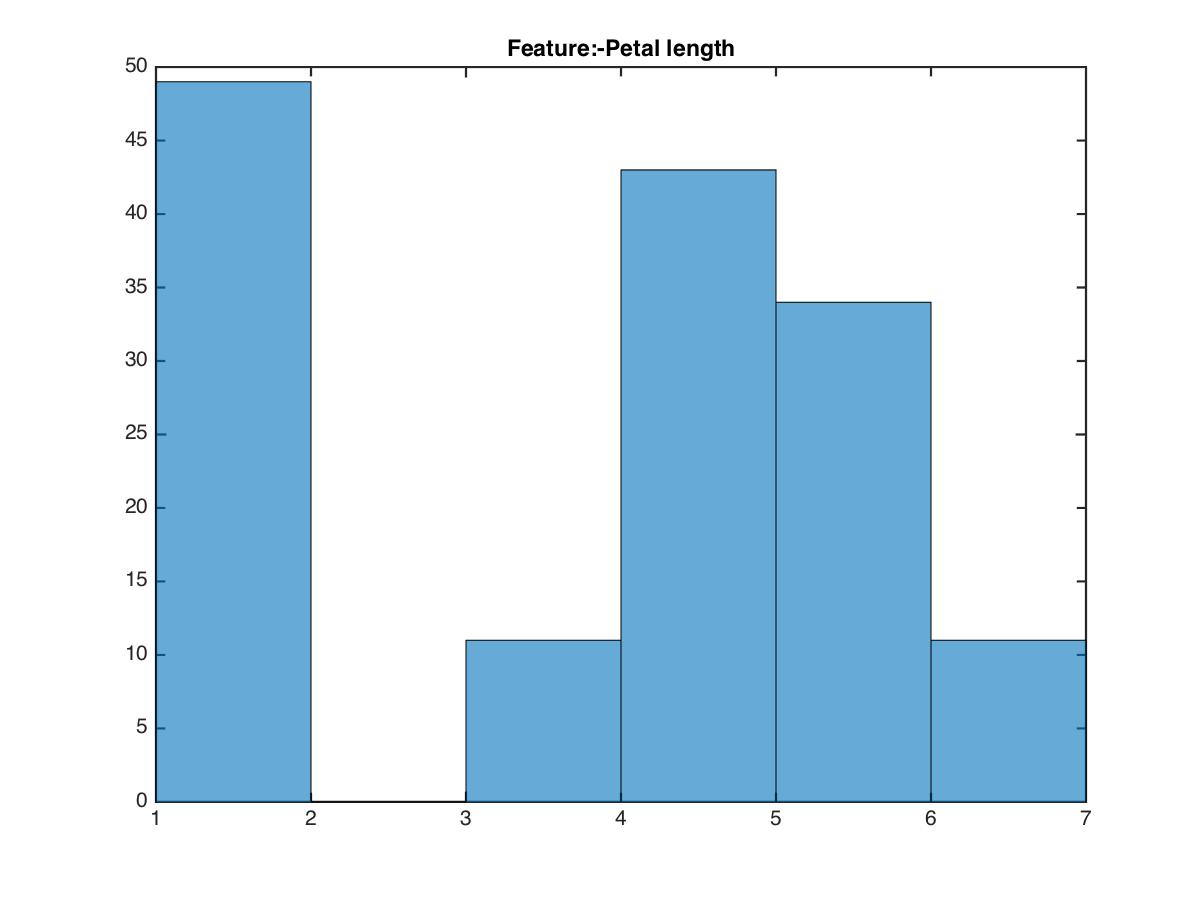
\includegraphics[scale=0.18]{histogram3.jpg}
}
\subfigure[Petal Width]{
    \label{fig:subfig4}
    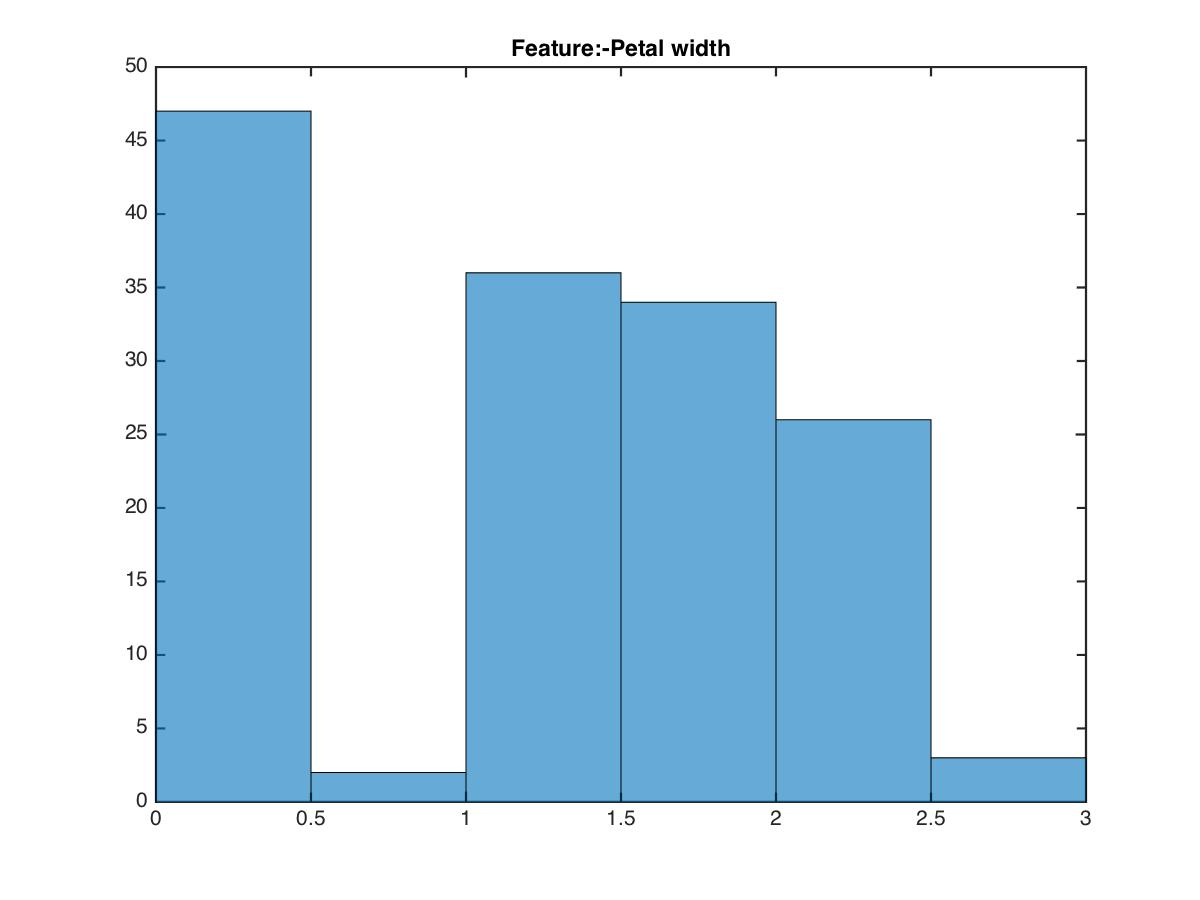
\includegraphics[scale=0.18]{histogram4.jpg}
}
\caption[Histogram1]{Histogram of features in the `Fisher iris' data set}
\label{fig:histogram1a}
\end{figure}

\begin{figure}
\centering
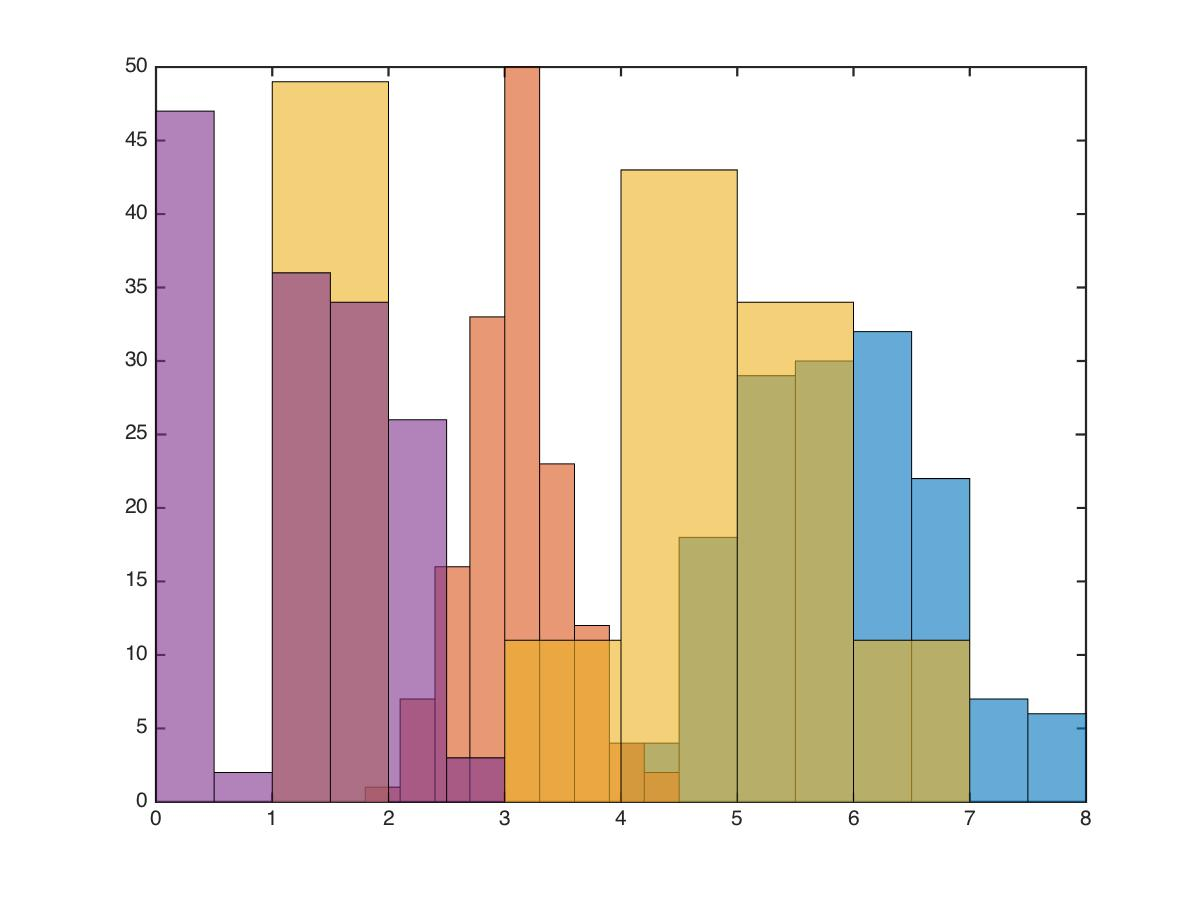
\includegraphics[scale=0.2]{histogram5.jpg}
\caption[Histogram2]{Histogram of features in the `Fisher iris' data set.}
\label{fig:histogram1b}
\end{figure}

%% Part (c)
\item The mean is computed using the \mcode{mean()} method provided by matlab (\autoref{lst:mean})
\vspace{-20pt}
\begin{lstlisting}[caption={Mean of features of `Fisher iris' data set.},label={lst:mean},numbers=left,escapeinside={@}{@}]
%% Part (c)
% Compute the mean of the data points for each feature (mean)
disp('Mean');
meanX = mean(X);
for f=1:size(X, 2);
    disp(strcat({'Feature:- '}, features(f,:),{': '} , num2str(meanX(:,f))));
end;

%Output
Mean
    'Feature:- Sepal length: 5.9001'
    'Feature:- Sepal width: 3.0989'
    'Feature:- Petal length: 3.8196'
    'Feature:- Petal width: 1.2526'
\end{lstlisting}

\item The mean is computed using the \mcode{mean()} method provided by matlab (\autoref{lst:mean})
\vspace{-20pt}
\begin{lstlisting}[caption={Mean of features of `Fisher iris' data set.},label={lst:mean},numbers=left,escapeinside={@}{@}]
%% Part (d)
% Compute the variance and standard deviation of the data points for each feature
disp('Standard Deviations')
stdX = std(X);
for f=1:size(X, 2);
    disp(strcat({'Feature:- '}, features(f,:),{': '} , num2str(stdX(:,f))));
end;

disp('Variances')
varX = var(X);
for f=1:size(X, 2);
    disp(strcat({'Feature:- '}, features(f,:),{': '} , num2str(varX(:,f))));
end;

%Output
Standard Deviations
    'Feature:- Sepal length: 0.83623'
    'Feature:- Sepal width: 0.43777'
    'Feature:- Petal length: 1.76'
    'Feature:- Petal width: 0.76135'

Variances
    'Feature:- Sepal length: 0.69928'
    'Feature:- Sepal width: 0.19165'
    'Feature:- Petal length: 3.0976'
    'Feature:- Petal width: 0.57965'
\end{lstlisting}

% Part (e)
\item I normalized the dataset using the \mcode{bsxfun()}, which applies element-by-element binary operations on the specified function. The functions I used were \mcode{@minus} and \mcode{@rdivide}. The code described in \autoref{lst:norm} shows the use. One more approach to achieve the same is seen in \autoref{lst:norm2}.
\vspace{-20pt}
\begin{lstlisting}[caption={Normalizing the data set},label={lst:norm},numbers=left,escapeinside={@}{@}]
% bsxfun: applies the element-by-element binary operation specified by the function handle fun to arrays A and B, with singleton expansion enabled.
normX = bsxfun(@rdivide, bsxfun(@minus, X, mean(X)), std(X));
\end{lstlisting}
\vspace{-20pt}
\begin{lstlisting}[caption={Normalizing the data set using \mcode{repmat()}},label={lst:norm2},numbers=left,escapeinside={@}{@}]
%One More way to do this (more understandable way) -
meanXMat = repmat(meanX, size(X,1),1); stdXMat = repmat(stdX, size(X,1),1);
norX1 = X - meanXMat; normX = norX1 ./ stdXMat;
\end{lstlisting}

\item The plot for pairs of features (1,2), (1,3), and (1,4) is created using a for-loop and the \mcode{scatter()}. The colors are set by passing the class values to the scatter function. The code that performs the operation can be seen in \autoref{lst:norm} and the resulting set of plots generated can be seen in \autoref{fig:norm1}
\vspace{-20pt}
\begin{lstlisting}[caption={Generating scatter plots for feature pairs - (1,2), (1,3), and (1,4).},label={lst:norm},numbers=left,escapeinside={@}{@}]
h=figure;
i = 1;

for f=2:size(X, 2);
    subplot(1,3,i);
    h1 = scatter(X(:,1), X(:,f), 50, y, 'filled');
    i = i+1;
    title(strcat({'X: '},features_short(1,:), {',Y:'}, features_short(f,:)))
    hold on;    
end;

hold off;
saveas(h,'plots.jpg','jpg');
\end{lstlisting}

\begin{figure}
\centering
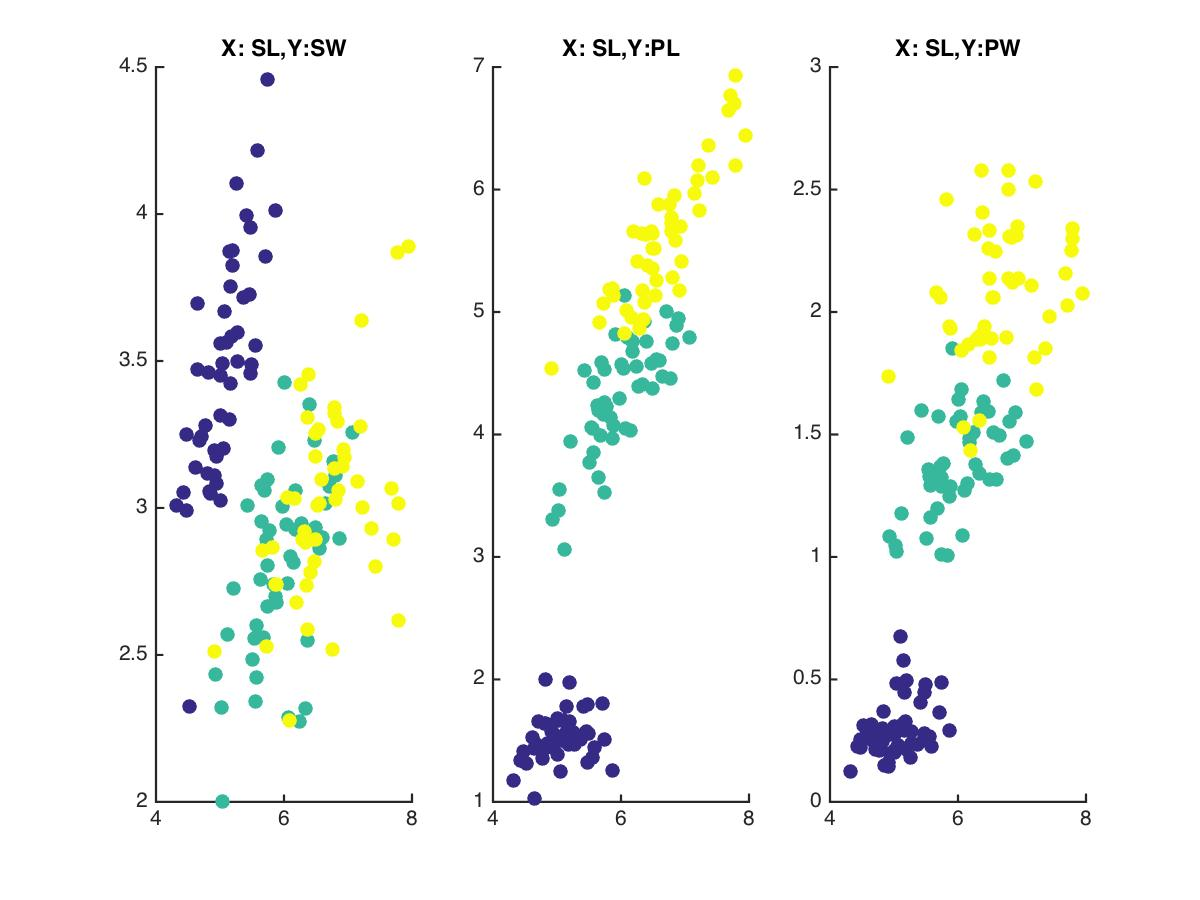
\includegraphics[scale=0.25]{plots.jpg}
\caption[norm1]{Plots generated with the feature pairs - (1,2), (1,3), and (1,4).}
\label{fig:norm1}
\end{figure}

\end{enumerate}
\vspace{-10pt}

%%%%%%%%%%%%%%%%%%%%%%%%%%%%%%%%%%%%%%%%%%%%%%%%%%%%%%%%%
%%%%%%%%%%%%%%%%%%%%%%%%%%%%%%%%%%%%%%%%%%%%%%%%%%%%%%%%%
\section*{Problem 2: kNN predictions}
\vspace{-10pt}
In this problem, I looked at knnClassify class and the features provided by it to classify data in the Iris dataset. The data is shuffle and split into training and test subsets. The question had 2 sub-questions:
\begin{enumerate}[(a)]
\item I modified the code snippet provided in the homework description and created the classifier. The code after modification is given in \autoref{lst:knnmod}. The classes for various values of \textit{k} can be seen in \autoref{fig:knnClasses}. The \mcode{Randstream()} function helps in giving a seed to the randomizer and helps in reproducing the results. The \mcode{shuffleData()} was modified for accommodating the same with an option of being empty, in which the results would be generated randomly.
\vspace{-20pt}
\begin{lstlisting}[caption={Computes the classes using kNNClassify class and generates the scatter plot.},label={lst:knnmod},numbers=left,escapeinside={@}{@}]
i = 1;
for k=[1, 5, 10, 50];
    h=figure;
    %subplot(2,2,i);
    i = i+1;
    knn = knnClassify( Xtr, Ytr, k );
    YteHat = predict( knn, Xte ); 
    plotClassify2D( knn, Xtr, Ytr );
    title(strcat({'K= '},num2str(k)))
    saveas(h,strcat('2a-',num2str(k),'.jpg'),'jpg');
    hold on;
end;
hold off;
\end{lstlisting}

\begin{figure}
\centering
\subfigure[kNN boundaries for K=1]{
    \label{fig:subfig1}
    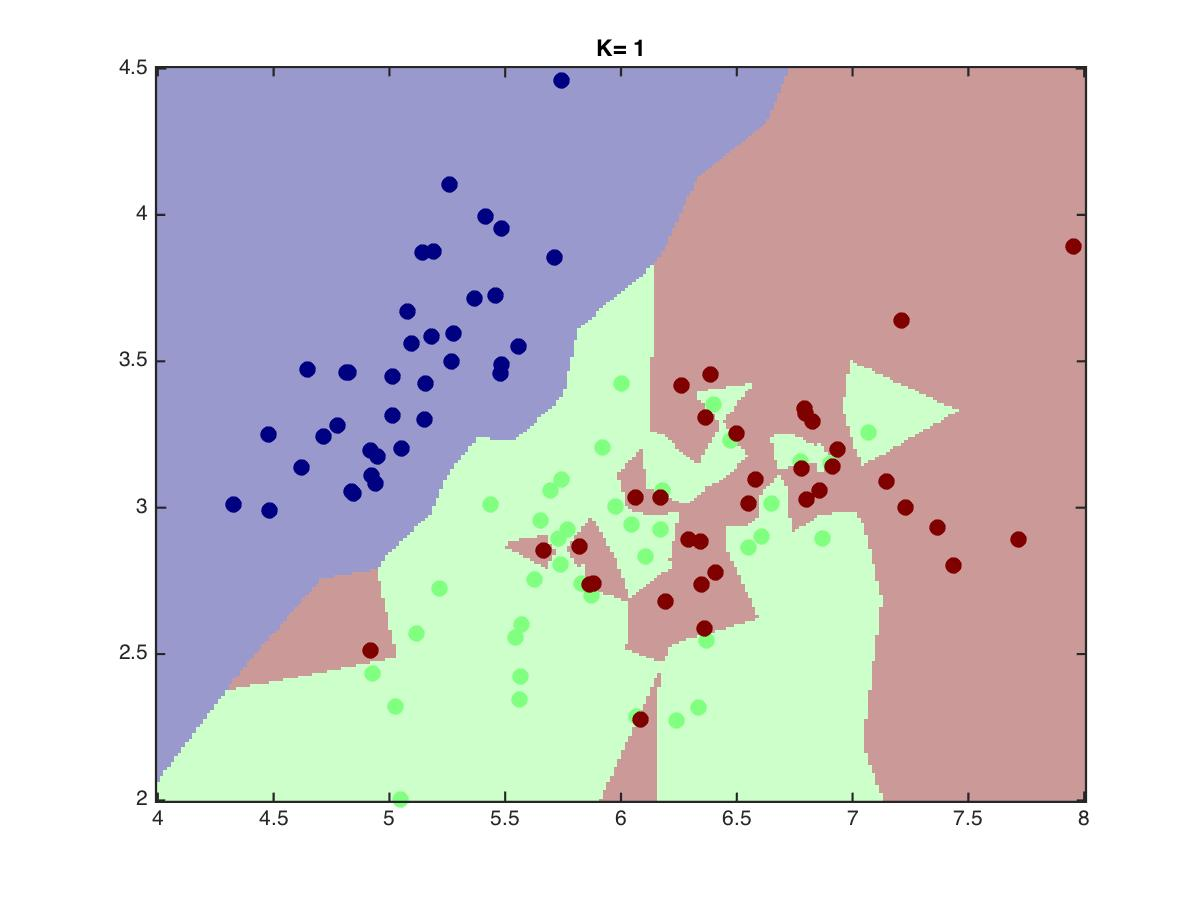
\includegraphics[scale=0.14]{2a-1.jpg}
}
\subfigure[kNN boundaries for K=5]{
    \label{fig:subfig2}
    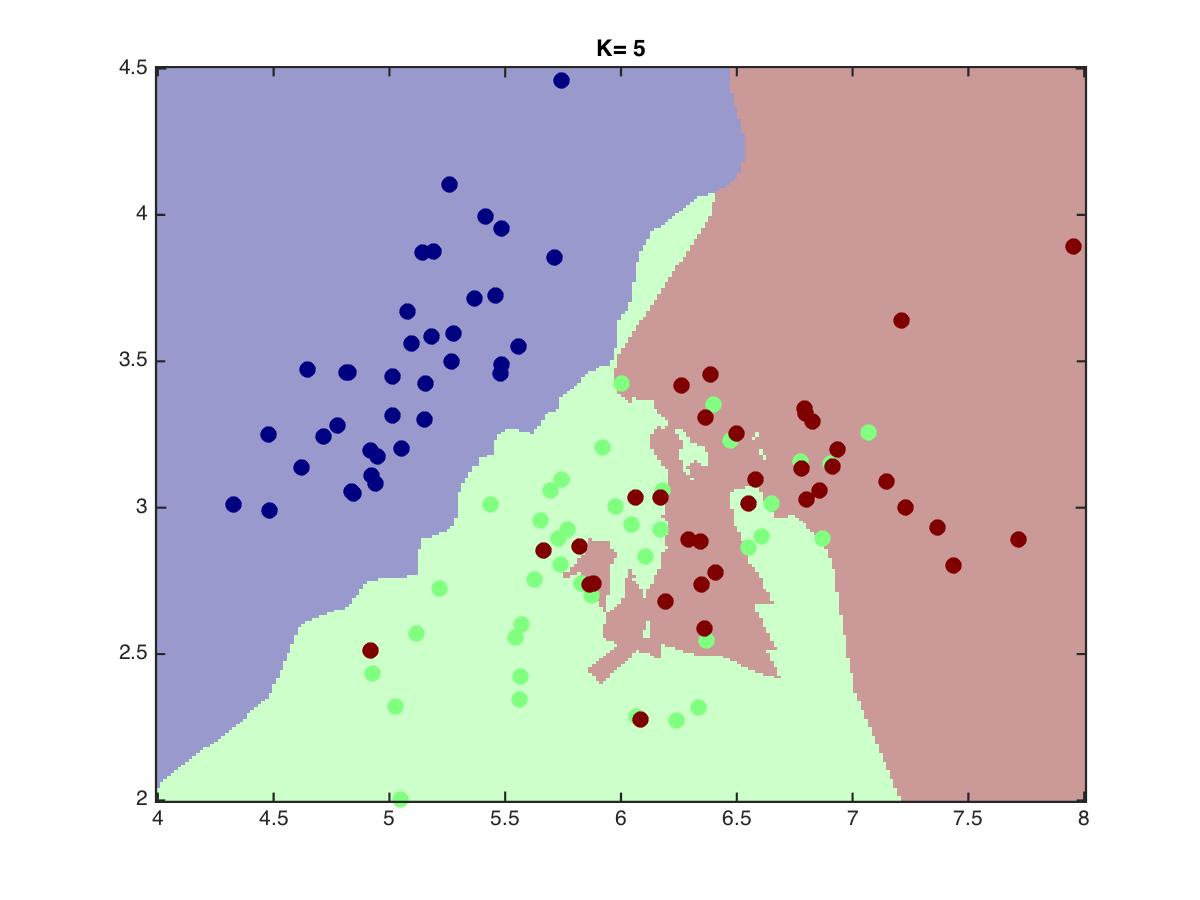
\includegraphics[scale=0.14]{2a-5.jpg}
}
\subfigure[kNN boundaries for K=10]{
    \label{fig:subfig3}
    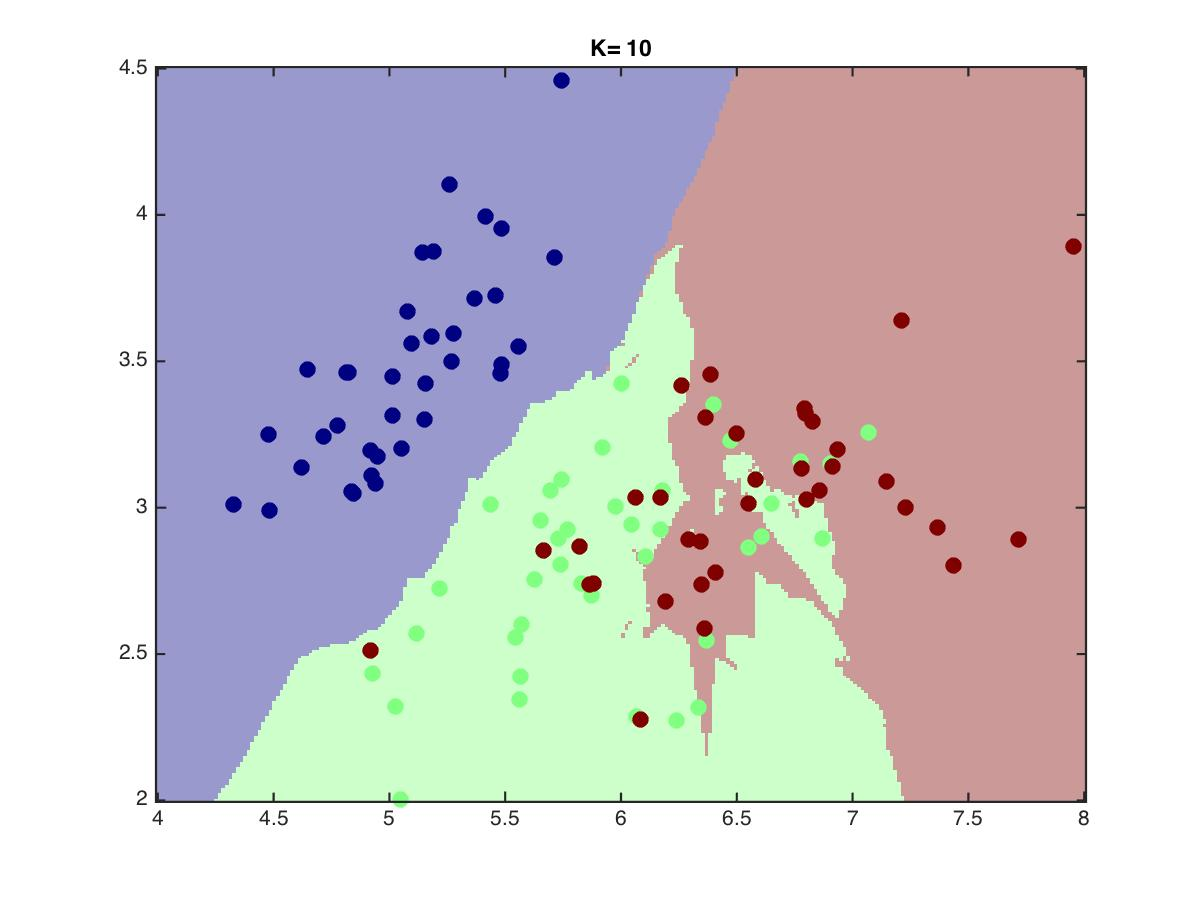
\includegraphics[scale=0.14]{2a-10.jpg}
}
\subfigure[kNN boundaries for K=50]{
    \label{fig:subfig4}
    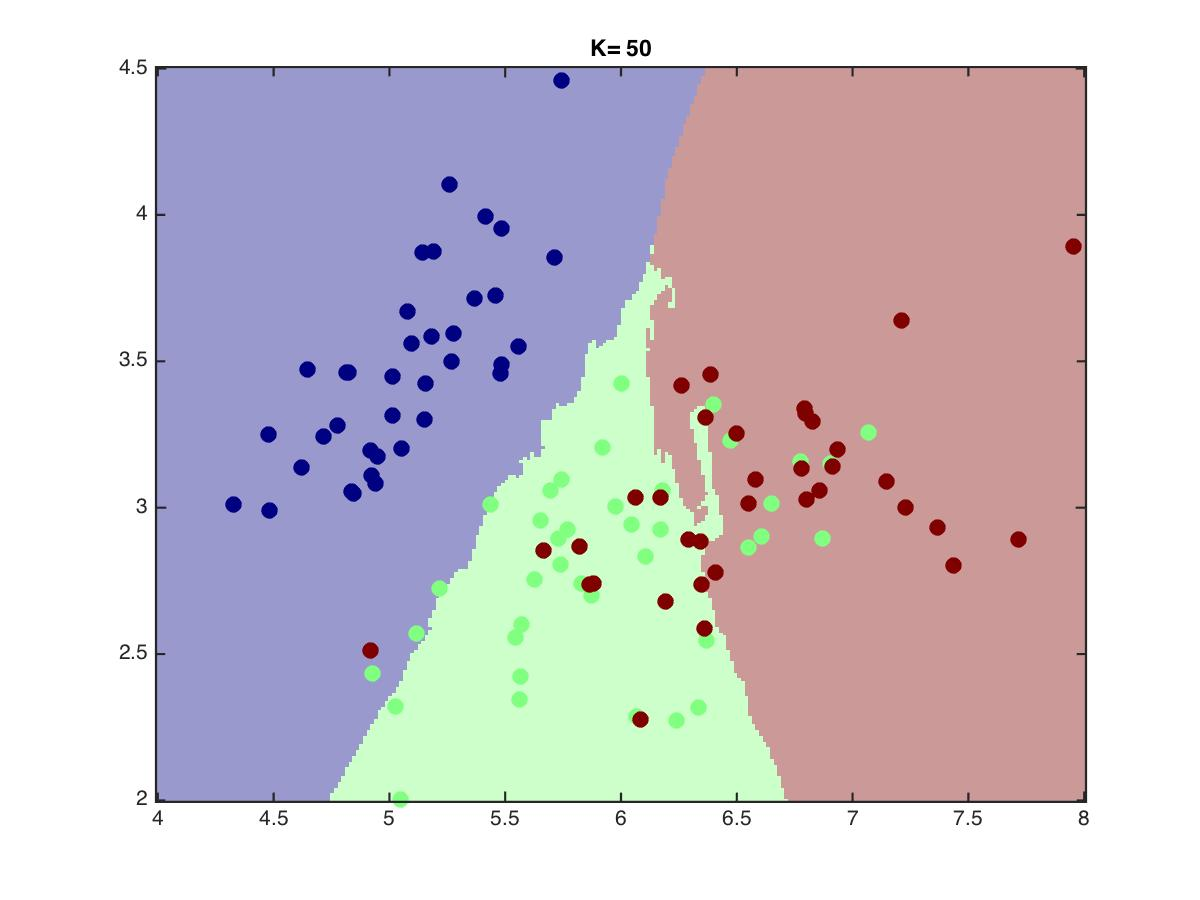
\includegraphics[scale=0.14]{2a-50.jpg}
}
\caption[knnClasses]{kNN Classifier output for various values of k.}
\label{fig:knnClasses}
\end{figure}

\item The error is computed using a different function \mcode{errorTrain()}, which compares the expected and actual assigned classes and checks for the matches. \mcode{errorTrain()} is described in \autoref{lst:errortrain}. \autoref{lst:errortrain2} describes the whole approach to solve the problem given. I used the \mcode{semilogx} based graph to present the test-vs-train error plotting for various values of \textit{k} and got \textit{k} = 50 to be a good value, as also shown by \autoref{fig:errorrate}. Also to understand the graph in a better way, I changed the value of \textit{k} to a range of 1 to 100. The results of this are portrayed in \autoref{fig:errorrate2}. It is very similar to the one showed in the class and portrays the overfitting and underfitting zones well.
\vspace{-20pt}
\begin{lstlisting}[caption={\mcode{errorTrain()} to compute the error in the classes assigned.},label={lst:errortrain},numbers=left,escapeinside={@}{@}]
function [error] = errorTrain(Yte, YteHat)
% Y = from1ofK(Y1k [,values]) : convert 1-of-K valued Y into discrete representation
%  optional "values" specifies the possible values of Y (default 1..K)

error = 0;
for i=1:size(Yte,1);
    if(Yte(i) ~= YteHat(i));
        error = error + 1;
    end;
end;

error = error/size(Yte,1);
\end{lstlisting}
\vspace{-20pt}
\begin{lstlisting}[caption={Code to generate the \mcode{semilogx} classifier error graphs},label={lst:errortrain2},numbers=left,escapeinside={@}{@}]
%% Part (b)
% Training with Xtr and Ytr
K=[1,2,5,10,50,100,200, 300];
errorsTr = zeros(size(K));
errorsTe = zeros(size(K));
for i=1:size(K,2);
    knn = knnClassify( Xtr, Ytr, K(:,i));
    YtrHat = predict( knn, Xtr );
    errorsTr(1,i) = errorTrain(Ytr, YtrHat);
    YteHat = predict( knn, Xte );
    errorsTe(1,i) = errorTrain(Yte, YteHat);
end;

h=figure;
semilogx(log(K), errorsTr);
hold on;
semilogx(log(K), errorsTe);
hold off;

disp(K(find(errorsTe == min(errorsTe))));
    50
\end{lstlisting}
\begin{figure}
\centering
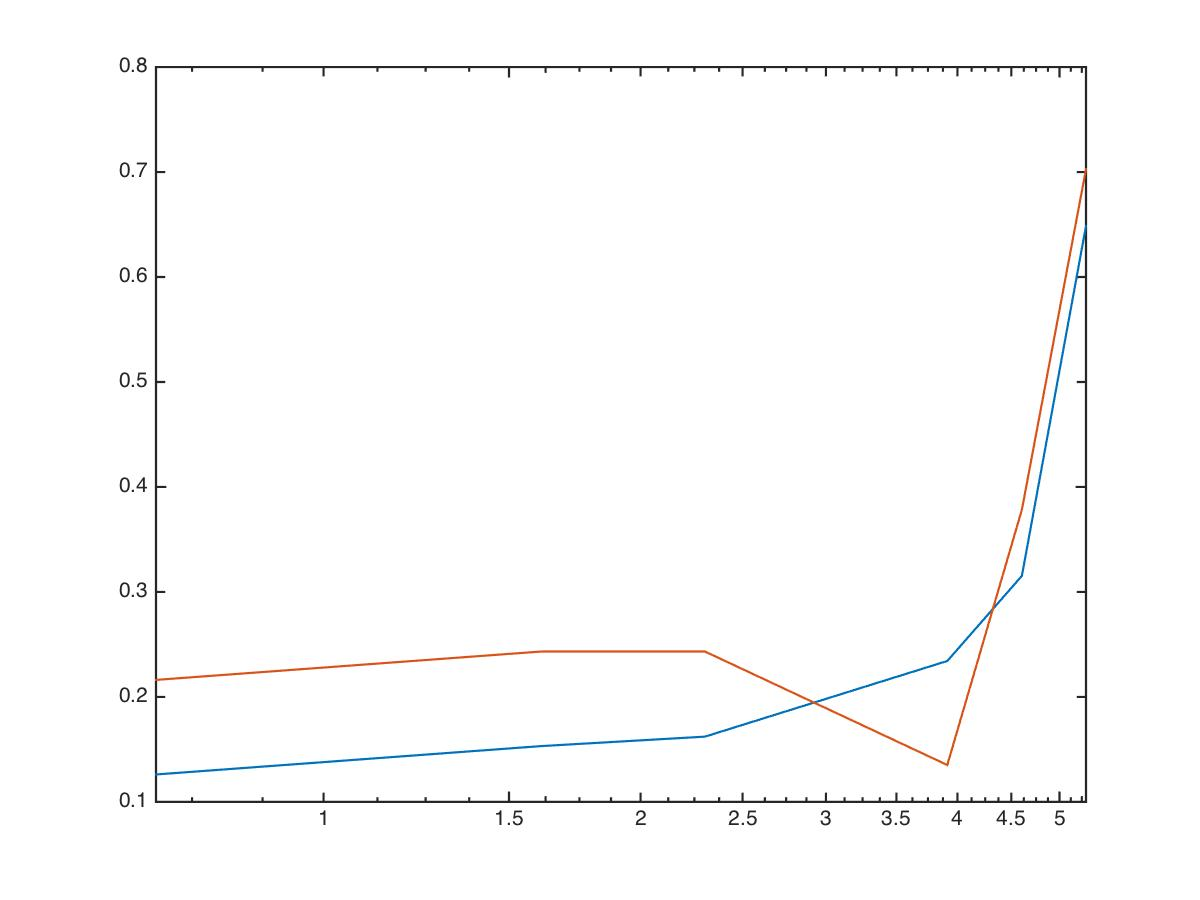
\includegraphics[scale=0.25]{errorrate.jpg}
\caption[Error2]{Resulting error rate functions using a semi-log plot with training errors in green and testing error in red for \textit{k} = [1,2,5,10,50,100,200].}
\label{fig:errorrate}
\end{figure}
\begin{figure}
\centering
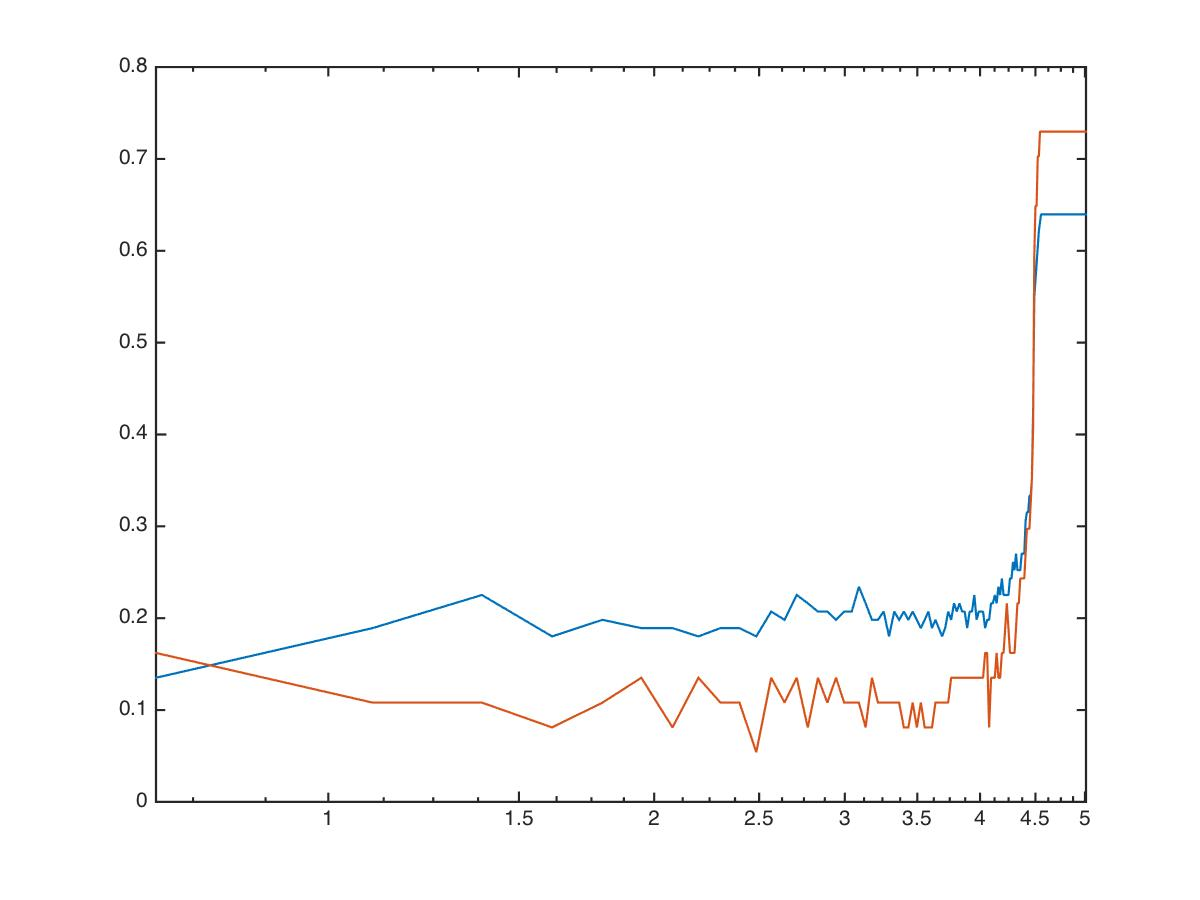
\includegraphics[scale=0.25]{errorrate2.jpg}
\caption[Error3]{Resulting error rate functions using a semi-log plot with training errors in green and testing error in red for \textit{k} = 1:100.}
\label{fig:errorrate2}
\end{figure}
\end{enumerate}
\vspace{-10pt}
%%%%%%%%%%%%%%%%%%%%%%%%%%%%%%%%%%%%%%%%%%%%%%%%%%%%%%%%%
%%%%%%%%%%%%%%%%%%%%%%%%%%%%%%%%%%%%%%%%%%%%%%%%%%%%%%%%%
\section*{Problem 3: Bayes Classifiers}
\begin{enumerate}[(a)]
\item I computed the 
\vspace{-20pt}
\begin{lstlisting}[caption={Calculating the necessary probabilities for Naive Bayes},label={lst:naivebayes1},numbers=left,escapeinside={@}{@}]
email_data = [0 0 1 1 0 -1;
     1 1 0 1 0 -1;
     0 1 1 1 1 -1;
     1 1 1 1 0 -1;
     0 1 0 0 0 -1;
     1 0 1 1 1 1;
     0 0 1 0 0 1;
     1 0 0 0 0 1;
     1 0 1 1 0 1;
     1 1 1 1 1 -1];
 
y = email_data(:,end);
X = email_data(:,1:end-1);
classes = unique(y);

[uniqClasses, numUniqClasses] = count_unique(y);
class_prob = zeros(size(uniqClasses)); % We'll calculate it later.
% class_prob(i, :) = numUniqClasses (i,:) / sum(numUniqClasses);

class_count = zeros(size(uniqClasses,1), size(X,2));

% Counting the occurances of Xi for different values of the classes
% For each feature - 
for xi = 1:size(X,2);
    [uniqX, numUniqX] = count_unique(X(:,xi));
    for xn = 1:size(X,1);
        if X(xn,xi) == 1;
            class_count(find(uniqClasses == y(xn)) , xi) = class_count(find(uniqClasses == y(xn)) , xi) + 1;
        end;
    end;
end;

% Gets the probabilities of the ones cases, where the data is 1.
probabilities_of_one_cases = zeros(size(class_count));
for col = 1:size(probabilities_of_one_cases, 2);
    for row = 1:size(probabilities_of_one_cases, 1);
        probabilities_of_one_cases(row,:) = class_count(row,:) ./ numUniqClasses (row);
    end;
end;

% Gets the probabilities of the zero cases, where the data is 0.
probabilities_of_zero_cases = 1 - probabilities_of_one_cases;

disp('probabilities_of_one_classes');
[probabilities_of_one_cases, uniqClasses]
disp('probabilities_of_zero_classes');
[probabilities_of_zero_cases, uniqClasses]

---------------------------------------
probabilities_of_one_classes
ans =
    0.5000    0.8333    0.6667    0.8333    0.3333   -1.0000
    0.7500         0    0.7500    0.5000    0.2500    1.0000

probabilities_of_zero_classes
ans =
    0.5000    0.1667    0.3333    0.1667    0.6667   -1.0000
    0.2500    1.0000    0.2500    0.5000    0.7500    1.0000
\end{lstlisting}

\item For computing the class using the Naive Bayes classifier, we used the basic code used in the previous question (\autoref{lst:naivebayes1}) and computing it by calculating the chance of the class being one of the given classes (+1 and -1 in our example). The code to compute the associated class is given in \autoref{lst:naivebayesexample1}. 
\begin{itemize}
\item For input = [0, 0, 0, 0, 0]: The computed class of the email is 1 with a probability of 0.8351. The system would recommended this email to be read.
\item For input = [1, 1, 0, 1, 0]: The computed class of the email is -1 with a probability of 1. The system would recommended this email to not be read.
\end{itemize}
\vspace{-20pt}
\begin{lstlisting}[caption={For some input},label={lst:naivebayesexample1},numbers=left,escapeinside={@}{@}]
% 
% P(y|X) = p(X|y) p(y) / P(X)
% P(y = -1 |X) = p(X|y = -1) p(y = -1) / P(X)

% P(y = -1 |X) = 
% p(X|y = -1) p(y = -1)
% ------------------------------------
%(p(X|y=-1) p(y=-1) + p(X|y=1) p(y=1))

% P(y = 1 |X) = 
% p(X|y = 1) p(y = 1)
% ------------------------------------
%(p(X|y=-1) p(y=-1) + p(X|y=1) p(y=1))

input = [0, 0, 0, 0, 0];
% input = [1, 1, 0, 1, 0];

% finding the classes for -1
productClass1 = 1;
for i = 1:size(input,2); 
    if input(:,i) == 1;
       productClass1 = productClass1 *  probabilities_of_one_cases(1,i);
    else
       productClass1 = productClass1 *  probabilities_of_zero_cases(1,i);
    end;
end;

% finding the classes for 1
productClass2 = 1;
for i = 1:size(input,2);
    if input(:,i) == 1;
       productClass2 = productClass2 *  probabilities_of_one_cases(2,i);
    else
       productClass2 = productClass2 *  probabilities_of_zero_cases(2,i);
    end;
end;

probClass1 = productClass1 * class_prob(1,:) / (productClass1 * class_prob(1,:) + productClass2 * class_prob(2,:));
probClass2 = productClass2 * class_prob(2,:) / (productClass1 * class_prob(1,:) + productClass2 * class_prob(2,:));
\end{lstlisting}

\item The posterior probability of y = +1 given X = [1, 1, 0, 1, 0] is 0. This corroborates with the fact that X was also a data point which the data was trained on, and its class with -1.

\item Using a Bayes classifier for such kind of data where there is high cost associated with false positives and false negatives can have high impact. Also, for very high number of features, not assuming independent features can be computationally very expensive as it would be a combinatorial explosion.
\end{enumerate}

%%%%%%%%%%%%%%%%%%%%%%%%%%%%%%%%%%%%%%%%%%%%%%%%%%%%%%%%%
%%%%%%%%%%%%%%%%%%%%%%%%%%%%%%%%%%%%%%%%%%%%%%%%%%%%%%%%%
\section*{Problem 4: Gaussian Bayes Classifiers}
\vspace{-5pt}
I used some of the features provided in the \mcode{gaussBayesClassify} class and was able to create  
\begin{enumerate}[(a)]
\item As before, I split data vertically to get the first 2 features of Iris dataset. After getting this data, I computed the number of unique classes and each ones count. This was done using the \mcode{count_unique()} function. This is previously used in Problem 3. Once I got the unique classes, I fetched all the indices from the training set which matched the class value and found the mean and covariance of the temporary matrices using the \mcode{mean()} and \mcode{cov()} functions of Matlab.
\vspace{-20pt}
\begin{lstlisting}[caption={Visualizeing the classifier and the boundaries},label={lst:gbayes1},numbers=left,escapeinside={@}{@}]
%% Part(a)
% Splitting by class
[tempUniq, numTemp] = count_unique(Ytr);
mean_matrix = zeros(size(tempUniq,1), size(Xtr,2));
for i = 1:size(tempUniq,1);
    temp = Xtr(find(Ytr==tempUniq(i,:)),:); % All the indexes of 
    disp(strcat('Class:',num2str(i)))
    disp('--------------------------------')
    mean_matrix (i,:) = mean(temp); % Mean Stored for future use
    disp('Mean of the class')
    disp(mean_matrix (i,:));
    disp('Covariance matrix')
    disp(cov(temp)); % Creating and displaying the Covariance matrix of the class data.
end;
\end{lstlisting}
\vspace{-20pt}
\begin{lstlisting}[caption={Output of the code from \autoref{lst:gbayes1}},label={lst:gbayes2},numbers=left,escapeinside={@}{@}]
Class:1
--------------------------------
Mean of the class
    5.0721    3.4765
Covariance matrix
    0.1194    0.0880
    0.0880    0.1159

Class:2
--------------------------------
Mean of the class
    5.9581    2.8093
Covariance matrix
    0.2967    0.0939
    0.0939    0.1138

Class:3
--------------------------------
Mean of the class
    6.5659    3.0264
Covariance matrix
    0.3730    0.1039
    0.1039    0.1039
\end{lstlisting}

\item The scatter plot generated by \autoref{lst:gbayes1} is given in \autoref{fig:scatter-bayes}.
\vspace{-20pt}
\begin{lstlisting}[caption={Visualizeing the classifier and the boundaries},label={lst:gbayes1},numbers=left,escapeinside={@}{@}]
h = figure;
scatter(Xtr(:,1), Xtr(:,2), 50, Ytr, 'filled');
saveas(h,'scatter-bayes.jpg','jpg');
\end{lstlisting}

\begin{figure}
\centering
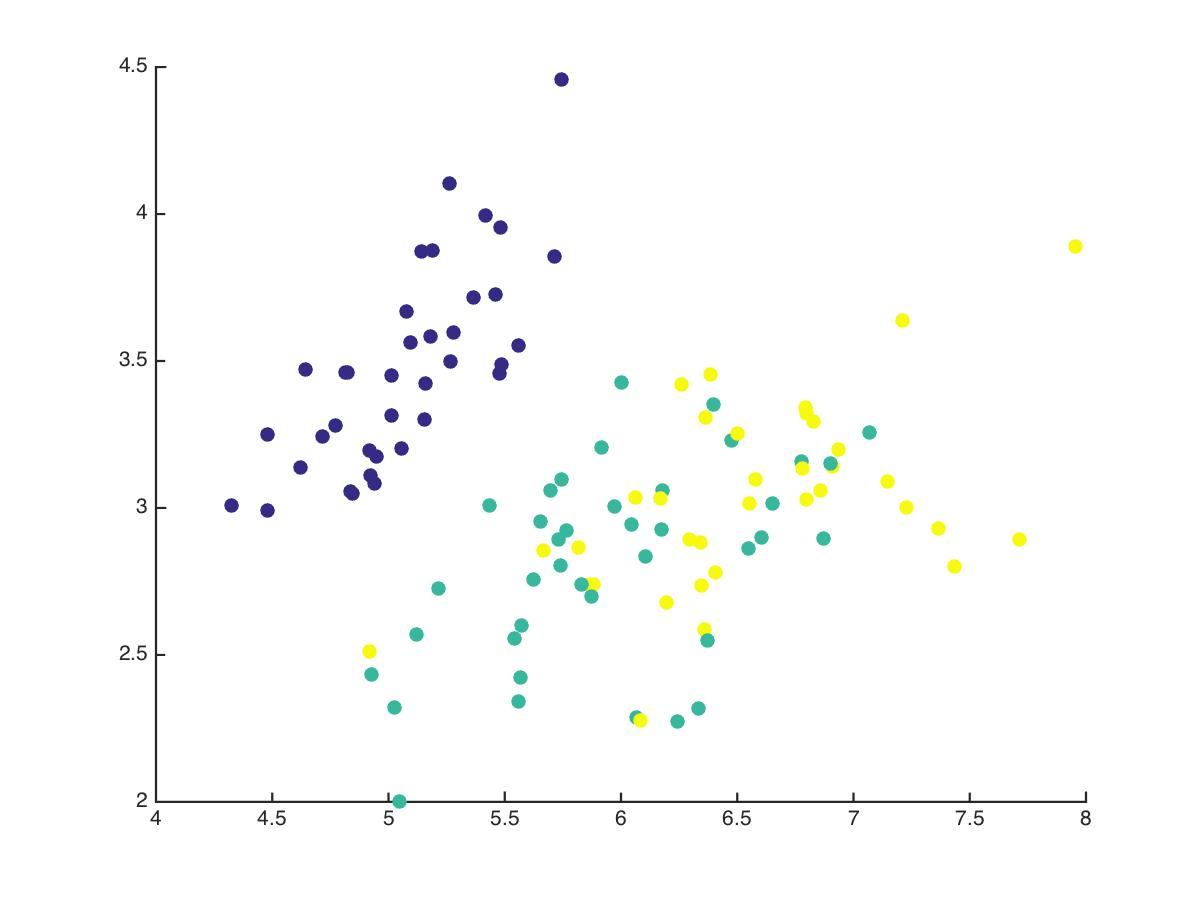
\includegraphics[scale=0.25]{scatter-bayes.jpg}
\caption[Scatter]{Scatter plot of Iris data set used Gaussian Bayes Learner.}
\label{fig:scatter-bayes}
\end{figure}

\item The scatter plot along with the contours based on the covariance matrix and the mean of data is generated by \autoref{lst:gbayes2} is given in \autoref{fig:scatter-bayes-2}.
\vspace{-20pt}
\begin{lstlisting}[caption={Visualizeing the classifier and the boundaries},label={lst:gbayes1},numbers=left,escapeinside={@}{@}]
% Evaluate each point of feature space and predict the class
[tempUniq, numTemp] = count_unique(Ytr);
mean_matrix = zeros(size(tempUniq,1), size(Xtr,2));
color = {'blue','green','yellow'};
figure;
scatter(Xtr(:,1),Xtr(:,2), 50, Ytr, 'filled');
hold on;
for i = 1:size(tempUniq,1);
    temp = Xtr(find(Ytr==tempUniq(i,:)),:); % All the indexes of 
    mean_matrix (i,:) = mean(temp); % Mean Stored for future use
    plotGauss2D(mean(temp),cov(temp), color{i});
    hold on;
end;
hold off;
\end{lstlisting}

\begin{figure}
\centering
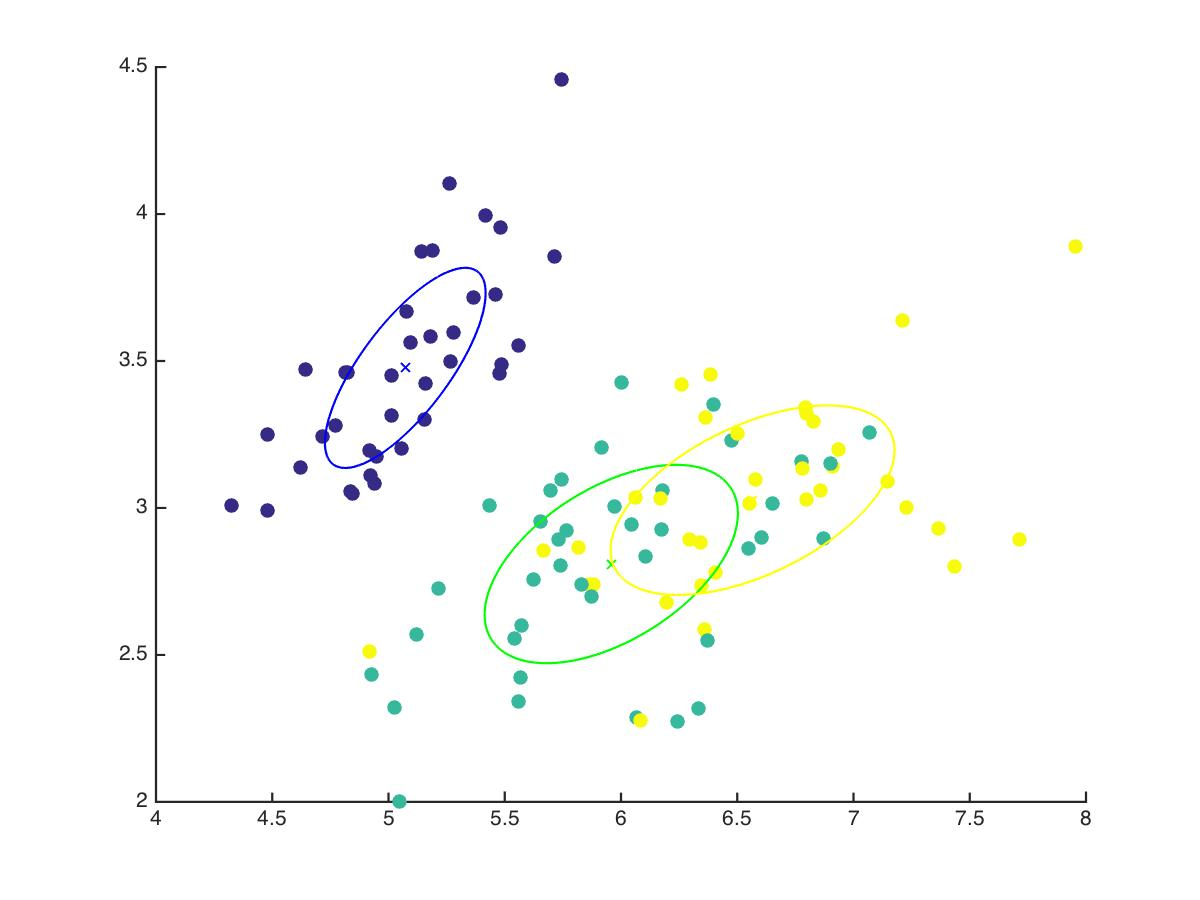
\includegraphics[scale=0.25]{scatter-bayes-2.jpg}
\caption[Scatter]{Scatter plot with counters of Iris data set.}
\label{fig:scatter-bayes-2}
\end{figure}

\item The code given in \autoref{lst:bayes2} generates the plot given in \autoref{fig:bayes2}.
\vspace{-20pt}
\begin{lstlisting}[caption={Visualizeing the classifier and the boundaries},label={lst:bayes2},numbers=left,escapeinside={@}{@}]
%% Part(d)
h = figure;
bc = gaussBayesClassify( Xtr, Ytr );
plotClassify2D(bc, Xtr, Ytr);
saveas(h,'bayes-2.jpg','jpg');
\end{lstlisting}
\begin{figure}
\centering
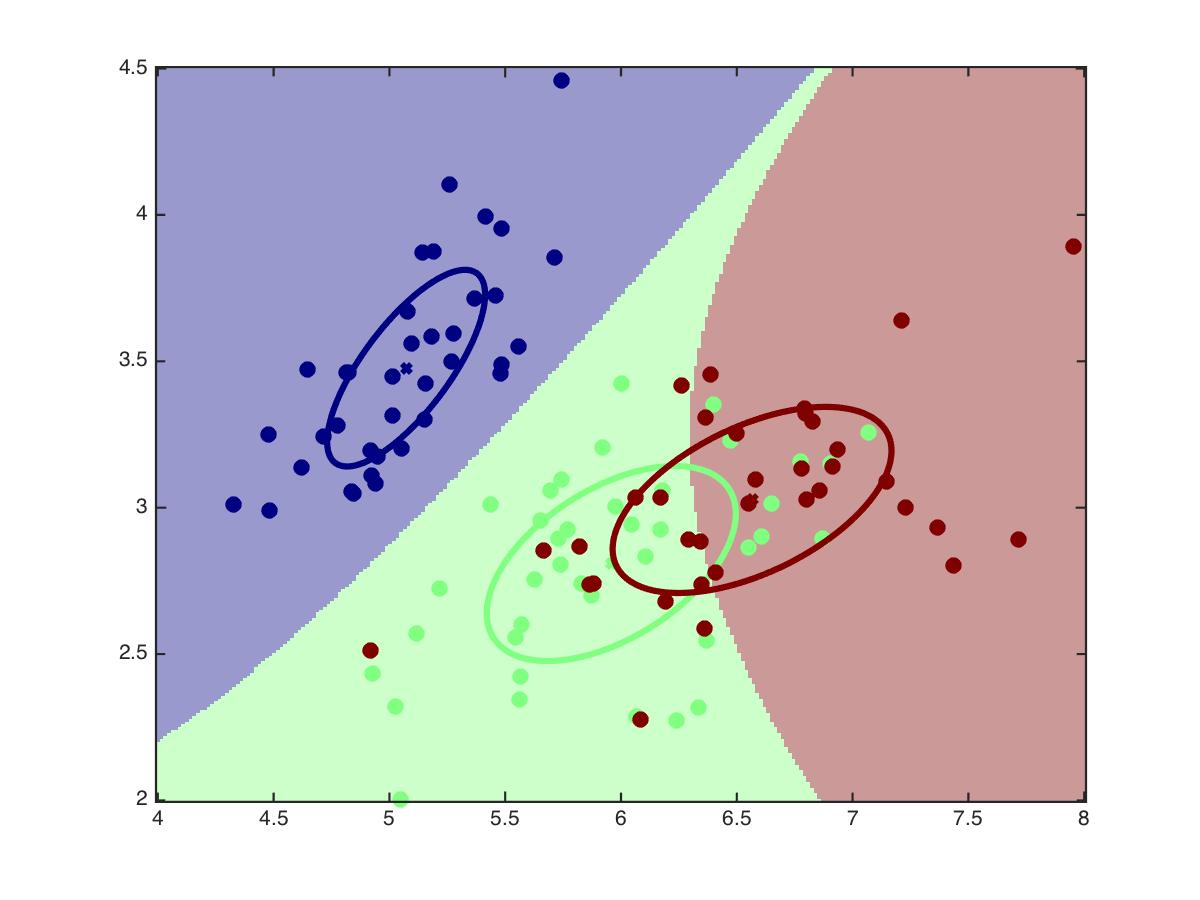
\includegraphics[scale=0.30]{bayes-2.jpg}
\caption[Bayes]{Bayes classifier in action: Generating the decision boundaries using Bayes classifier.}
\label{fig:bayes2}
\end{figure}

\item The code given in \autoref{lst:bayes3} computes the training error rate and the testing error rate. The code uses \mcode{errorTrainBayes()} to compute the number of misclassifications and the rate. It is a variant of \autoref{lst:errortrain}.
\vspace{-20pt}
\begin{lstlisting}[caption={Calculating the error rate.},label={lst:bayes3},numbers=left,escapeinside={@}{@}]
%% Part(e)
% Training error
bc = gaussBayesClassify( Xtr, Ytr );
YtrHat = predict( bc, Xtr );
[errorsCount, errorRate] = errorTrainBayes(Ytr, YtrHat);
>> [errorsCount, errorRate]
ans =
   23.0000    0.2072

% Testing error
bcTe = gaussBayesClassify( Xte, Yte );
YteHat = predict( bcTe, Xte );
[errorsCount, errorRate] = errorTrainBayes(Yte, YteHat);
>> [errorsCount, errorRate]
ans =
    9.0000    0.2432
\end{lstlisting}

\item When training the data with all the features of the data set, I saw tremendous improvement in the working of the classifier. It predicted all the test data results with 100\% accuracy. The code of the same is given in the \autoref{lst:bayes4}. I've put the output within the code itself.
\vspace{-20pt}
\begin{lstlisting}[caption={Bayesian classifier for all the 4 features of the Iris data set.},label={lst:bayes4},numbers=left,escapeinside={@}{@}]
%% Part(f)
bc = gaussBayesClassify( Xtr, Ytr );
YtrHat = predict( bc, Xtr );
[errorsCountTr, errorRateTr] = errorTrainBayes(Ytr, YtrHat);
[errorsCountTr, errorRateTr]
% Output
ans =
    2.0000    0.0180
    
bcTe = gaussBayesClassify( Xte, Yte );
YteHat = predict( bcTe, Xte );
[errorsCountTe, errorRateTe] = errorTrainBayes(Yte, YteHat);
[errorsCountTe, errorRateTe]
% Output
ans =
     0     0
\end{lstlisting}
\end{enumerate}
\end{document}

%%%%%%%%%%%%%%%%%%%%%%%%%%%%%%%%%%%%%%%%%%%%%%%%%%%%%%%%%
%%%%%%%%%%%%%%%%%%%%%%%%%%%%%%%%%%%%%%%%%%%%%%%%%%%%%%%%%
%%%%%%%%%%%%%%%%%%%%%%%%%%%%%%%%%%%%%%%%%%%%%%%%%%%%%%%%%
%%%%%%%%%%%%%%%%%%%%%%%%%%%%%%%%%%%%%%%%%%%%%%%%%%%%%%%%%
\iffalse
\begin{figure}
\centering
\subfigure[Puzzle 1]{
    \label{fig:subfig1}
    \includegraphics[scale=0.30]{g1.png}
}
\subfigure[Puzzle 2]{
    \label{fig:subfig2}
    \includegraphics[scale=0.30]{g2.png}
}
\subfigure[Puzzle 3]{
    \label{fig:subfig3}
    \includegraphics[scale=0.30]{g3.png}
}
\subfigure[Puzzle 4]{
    \label{fig:subfig4}
    \includegraphics[scale=0.30]{g4.png}
}
\subfigure[Puzzle 5]{
    \label{fig:subfig5}
    \includegraphics[scale=0.30]{g5.png}
}
\subfigure[Puzzle 6]{
    \label{fig:subfig6}
    \includegraphics[scale=0.30]{g6.png}
}
\caption[Running Various Experiments]{Running Various Experiments. The three bars are for Brute Force, I-Consistency and I-Consistency with MRV search. All the times given are in Seconds}
\label{fig:rungraphs}
\end{figure}

\begin{figure}
\centering
\includegraphics[scale=0.55]{Kakuro1.png}
\caption[Example Problem and Solution]{Example Problem and Solution}
\label{fig:kakuroExample}
\end{figure}
\fi